
\chapter*{The Diffusion Equation and Implicit Methods}
\addcontentsline{toc}{chapter}{The Diffusion Equation and Implicit Methods} 
\section*{Analytic approach to the Diffusion Equation}
\addcontentsline{toc}{section}{Analytic approach to the Diffusion Equation} 

Now let\rq s attack the diffusion equation
\begin{equation}\label{eq:71}
\frac{\partial T}{\partial t}=D \frac{\partial^{2} T}{\partial x^{2}}
\end{equation}
This equation describes how the distribution $T$ (often temperature) diffuses
through a material with a constant diffusion coefficient $D$. The diffusion equation
can be approached analytically via separation of variables by assuming that T is
of the form $T(x,t) = g(x)f(t)$. Plugging this form into the diffusion equation, we
find
\begin{equation}\label{eq:72}
\frac{1}{D} \frac{\dot{f}(t)}{f(t)}=\frac{g^{\prime \prime}(x)}{g(x)}
\end{equation}
The left-hand side depends only on time, while the right-hand side depends only
on space, so both sides must equal a constant, say $-a^2$. Thus, $f (t)$ must satisfy
\begin{equation}\label{eq:73}
\dot{f}(t)=-\gamma f(t)
\end{equation}
where $ \gamma = a^2 D$ so that $f(t)$ is
\begin{equation}\label{eq:74}
f(t)=e^{-\gamma t}
\end{equation}
Meanwhile $g(x)$ must satisfy
\begin{equation}\label{eq:75}
g^{\prime \prime}(x)+a^{2} g(x)=0
\end{equation}
If we specify edge-value boundary conditions so that $T(x = 0,t) = 0$ and $T(x =
L,t) = 0$ then the solution to Eq. \ref{eq:75} is simply
\begin{equation}\label{eq:76}
g(x) = \sin(ax)
\end{equation}

and the separation constant can take on the values $a = n \pi /L$, where n is an integer.
Any initial distribution $T(x,t = 0)$ that satisfies these boundary conditions can be
composed by summing these sine functions with different weights using Fourier
series techniques. Notice that higher spatial frequencies (i.e. large $n$) damp faster,
according to Eq. \ref{eq:74}. We already studied how to use separation of variables
computationally in the first several labs of this manual, so let\rq s move directly to
time-stepping methods for solving the diffusion equation.

\section*{Numerical approach: a first try}
\addcontentsline{toc}{section}{Numerical approach: a first try} 

Let\rq s try to solve the diffusion equation on a grid as we did with the wave equation.
If we finite difference the diffusion equation using a centered time derivative and
a centered second derivative in $x$ we get
\begin{equation}\label{eq:77}
\frac{T_{j}^{n+1}-T_{j}^{n-1}}{2 \tau}=\frac{D}{h^{2}}\left(T_{j+1}^{n}-2 T_{j}^{n}+T_{j-1}^{n}\right)
\end{equation}
Solving for $T_j^{n+1}$ to obtain an algorithm similar to leapfrog then gives

\begin{equation}\label{eq:78}
T_{j}^{n+1}=T_{j}^{n-1}+\frac{2 D \tau}{h^{2}}\left(T_{j+1}^{n}-2 T_{j}^{n}+T_{j-1}^{n}\right)
\end{equation}
There is a problem starting this algorithm because of the need to have T one time
step in the past ($T_j^{n+1}$), but even after we work around this problem this algorithm
turns out to be worthless. We won\rq t make you code it up, but if you did, you\rq d
find that no matter how small a time step $\tau$ you choose, you encounter the same
kind of instability that plagues staggered leapfrog when the step size got too big
(infinite zig-zags). Such an algorithm is called unconditionally unstable, and is an
invitation to keep looking. This must have been a nasty surprise for the pioneers
of numerical analysis who first encountered it. \\ 
For now, let\rq s sacrifice second-order accuracy to obtain a stable algorithm. If
we don\rq t center the time derivative, but use instead a forward difference we find
\begin{equation}\label{eq:79}
\frac{T_{j}^{n+1}-T_{j}^{n}}{\tau}=\frac{D}{h^{2}}\left(T_{j+1}^{n}-2 T_{j}^{n}+T_{j-1}^{n}\right)
\end{equation}
This algorithm has problems since the left side of Eq. \ref{eq:79} is centered at time $t_{n+/frac{1}{2}}$,while the right side is centered at time $t_n$. This makes the algorithm inaccurate, but it turns out that it is stable if $\tau$ is small enough. Solving for $T_j^{n+1}$ yields
\begin{equation}\label{eq:710}
T_{j}^{n+1}=T_{j}^{n}+\frac{D \tau}{h^{2}}\left(T_{j+1}^{n}-2 T_{j}^{n}+T_{j-1}^{n}\right)
\end{equation}
\begin{problem}\label{P7.1}
	\marginpar{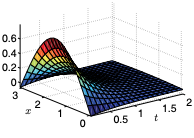
\includegraphics[width=\marginparwidth]{fig71}\captionof{figure}{Diffusion of the $n=$ 1 sine temperature distribution given in Problem \ref{P7.1}(a).}\label{fig:32}}
\begin{enumerate}[label=(\alph*)]
\item 
Modify one of your staggered leapfrog programs that uses a cell-center
grid to implement Eq. \ref{eq:710} to solve the diffusion equation on the
interval $[0,L]$ with initial distribution
\begin{equation}\label{eq:711}
T(x, 0)=\sin (\pi x / L)
\end{equation}

and boundary conditions $ T(0) = T (L) = 0$. Use $D = 2$, $L = 3$, and $N =
20$. You don\rq t need to make a space-time surface plot like Fig. 7.1. Just
make a line plot that updates each time step as we\rq ve done previously.
This algorithm has a CFL condition on the time step $\tau$ of the form

\begin{equation}\label{eq:712}
\tau \leq C \frac{h^{2}}{D}
\end{equation}
Determine the value of $C$ by numerical experimentation.
Test the accuracy of your numerical solution by overlaying a graph of
the analytic solution. Plot the numerical solution as points and the
exact solution as a line so you can tell the difference. Show that your
grid solution matches the exact solution with increasing accuracy as
the number of grid points $N$ is increased from 20 to 40 and then to 80.
You can calculate the RMS error using something like
\begin{lstlisting}
error = np.sqrt( np.mean( (T - exact)**2 ))
\end{lstlisting}

\item Get a feel for what the diffusion coefficient does by trying several
different values for $D$ in your code. Give a physical description of this
parameter to the TA.
\item Now switch your boundary conditions to be insulating, with $\partial T / \partial x=
0$ at both ends. Explain what these two types of boundary conditions
mean by thinking about a watermelon that is warmer in the middle
than at the edge. Tell physically how you would impose both of these
boundary conditions (specifying the value and specifying the derivative) on the watermelon and explain what the temperature history of
the watermelon has to do with your plots of $T(x)$ vs. time.
\end{enumerate}
\end{problem}
	\marginpar{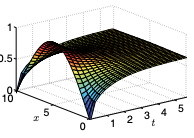
\includegraphics[width=\marginparwidth]{fig72}\captionof{figure}{Diffusion of the Gaussian temperature distribution given in Problem \ref{P7.1} (c) with insulating boundary conditions.}\label{fig:32}}
Even though this technique can give us OK results, the time step constraint for this
method is onerous. The constraint is of the form $\tau < C h^2$, where $C$ is a constant.
Suppose, for instance, that to resolve some spatial feature you need to decrease $h$
by a factor of 5; then you will have to decrease $\tau$ by a factor of 25. This will make
your code take forever to run, which motivates us to find a better way

\section*{Implicit Methods: the Crank-Nicolson Algorithm}
\addcontentsline{toc}{section}{Implicit Methods: the Crank-Nicolson Algorithm} 

The time-stepping algorithms we have discussed so far are of the same type: at
each spatial grid point $j$ you use present, and perhaps past, values of $y(x,t)$ at that
grid point and at neighboring grid points to find the future $y(x,t)$ at $j$. Methods
like this, that depend in a simple way on present and past values to predict future
values, are said to be $explicit$ and are easy to code. They are also often numerically
unstable, or have severe constraints on the size of the time step.\\
$Implicit$ methods are generally harder to implement than explicit methods,
but they have much better stability properties. The reason they are harder is that
they assume that you already know the future. To give you a better feel for what\rq\rq implicit\lq\lq means, let\rq s study the simple first-order differential equation
\marginpar{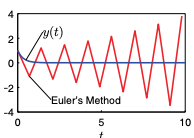
\includegraphics[width=\marginparwidth]{fig73}\captionof{figure}{Euler\rq s method is unstable for $\tau>2 .$ ( $\tau=2.1$ in this case.)}\label{fig:33}}

\begin{equation}\label{eq:713}
\frac{dy}{dt	} = -y
\end{equation}
\begin{problem}\label{P7.2}
\begin{enumerate}[label=(\alph*)]
\item Write a program to solve this equation using Euler\rq s method:
\begin{equation}\label{eq:714}
\frac{y_{n+1}-y_n}{\tau} = -y_n
\end{equation}
The program to solve for $y$ using Euler\rq s method is only a few lines of
code (like less than 10 lines, including the plot command). Here are
the first few lines:
\begin{lstlisting}
tau = 0.5
tmax = 20.
t = np.arange(0,tmax,tau)
y = np.zeros_like(t)
\end{lstlisting}
\marginpar{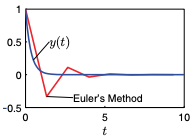
\includegraphics[width=\marginparwidth]{fig74}\captionof{figure}{Euler\rq s method is unstable for $\tau>2 .$ ( $\tau=2.1$ in this case.)}\label{fig:34}}

Show by numerical experimentation that Euler\rq s method is unstable
for large $\tau$ . You should find that the algorithm that is unstable if $\tau > 2$.
Use $y(0) = 1$ as your initial condition. This is an example of an explicit
\item Notice that the left side of Eq. \ref{eq:714} is centered on time $t_{n+\frac{1}{2}}$ but the
right side is centered on $t_n$. Fix this by centering the right-hand side at time $t_{n+\frac{1}{2}}$ by using an average of the advanced and current values of $y$, method.
\begin{equation*}
y_{n} \Rightarrow \frac{y_{n}+y_{n+1}}{2}
\end{equation*}
Modify your program to implement this fix, then show by numerical
experimentation that when $\tau$ becomes large this method doesn\rq t blow
up. It isn\rq t correct because $y_n$ bounces between positive and negative
values, but at least it doesn\rq t blow up. The presence of $\tau$ in the denominator is the tip-off that this is an implicit method, and the improved
stability is the point of using something implicit.
\marginpar{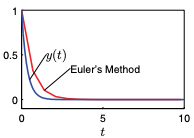
\includegraphics[width=\marginparwidth]{fig75}\captionof{figure}{The fully implicit method in $7.2(\mathrm{c})$ with $\tau=2.1$.}\label{fig:35}}

\item  Now Modify Euler\rq s method by making it fully implicit by using $y_{n+1}$
in place of $y_n$ on the right side of Eq. \ref{eq:714} (this makes both sides of
the equation reach into the future). This method is no more accurate
than Euler\rq s method for small time steps, but it is much more stable
and it doesn\rq t bounce between positive and negative values.
Show by numerical experimentation in a modified program that this
fully implicit method damps even when $ \tau $ is large. For instance, see
what happens if you choose $ \tau = 5$ with a final time of 20 seconds. The
time-centered method of part (b) would bounce and damp, but you
should see that the fully implicit method just damps. It\rq s terribly inaccurate, and actually doesn\rq t even damp as fast as the exact solution,
but at least it doesn\rq t bounce like part (b) or go to infinity like part (a).
Methods like this are said to be \rq\rq absolutely stable\lq\lq. Of course, it makes
no sense to choose really large time steps, like $ \tau = 100$ when you only
want to run the solution out to 10 seconds.

\end{enumerate}
\end{problem}
\section*{The diffusion equation with Crank-Nicolson}
\addcontentsline{toc}{section}{The diffusion equation with Crank-Nicolson} 
	\marginpar{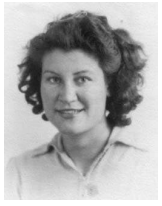
\includegraphics[width=\marginparwidth]{nicolson}\captionof{figure}{Phyllis Nicolson (1917-1968, English)}\label{fig:36}}
		
Now let\rq s look at the diffusion equation again and see how implicit methods can
help us find a stable numerical algorithm. Here\rq s the equation again
\begin{equation}\label{eq:715}
\frac{\partial T}{\partial t}=D \frac{\partial^{2} T}{\partial x^{2}}
\end{equation}
We begin by finite differencing the right side as usual:

\begin{equation}\label{eq:716}
\frac{\partial T_{j}}{\partial t}=D \frac{T_{j+1}-2 T_{j}+T_{j-1}}{h^{2}}
\end{equation}
Now we discretize the time derivative by taking a forward time derivative on the
left:
\begin{equation}\label{eq:717}
\frac{T_{j}^{n+1}-T_{j}^{n}}{\tau}=D \frac{T_{j+1}^{n}-2 T_{j}^{n}+T_{j-1}^{n}}{h^{2}}
\end{equation}
This puts the left side of the equation at time level $t_{n+\frac{1}{2}}$, while the right side is
at tn. To put the right side at the same time level (so that the algorithm will be
second-order accurate), we replace each occurrence of $T$ on the right-hand side
by the average

\begin{equation}\label{eq:718}
T^{n+\frac{1}{2}}=\frac{T^{n+1}+T^{n}}{2}
\end{equation}
like this:
\begin{equation}\label{eq:719}
\frac{T_{j}^{n+1}-T_{j}^{n}}{\tau}=D \frac{T_{j+1}^{n+1}+T_{j+1}^{n}-2 T_{j}^{n+1}-2 T_{j}^{n}+T_{j-1}^{n+1}+T_{j-1}^{n}}{2 h^{2}}
\end{equation}
If you look carefully at this equation you will see that there is a problem: how are
we supposed to solve for $T^{n+1}_j$? The future values $T^{n+1}$are all over the place, and
they involve three neighboring grid points ($T^{n+1}_{j-1}$ , $T^{n+1}_{j}$, and $T^{n+1}_{j+1}$) so we can’t just
solve in a simple way for $T^{n+1}_j$. This is an example of why implicit methods are
harder than explicit methods. \\ 
In the hope that something useful will turn up, let\rq s put all of the variables at
time level $n +1$ on the left, and all of the ones at level n on the right.
\marginpar{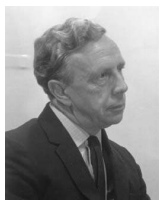
\includegraphics[width=\marginparwidth]{crank}\captionof{figure}{John Crank (1916-2006, English)}\label{fig:37}}

\begin{equation}\label{eq:720}
-T_{j-1}^{n+1}+\left(\frac{2 h^{2}}{\tau D}+2\right) T_{j}^{n+1}-T_{j+1}^{n+1}=T_{j-1}^{n}+\left(\frac{2 h^{2}}{\tau D}-2\right) T_{j}^{n}+T_{j+1}^{n}
\end{equation}
We know this looks ugly, but it really isn\rq t so bad. To solve for $T^{n+1}_j$we just need to
solve a linear system, as we did in Lab 2 on two-point boundary value problems.
When a system of equations must be solved to find the future values, we say
that the method is implicit. This particular implicit method is called the CrankNicolson algorithm. \\ 
To see more clearly what we are doing, and to make the algorithm a bit more
efficient, let\rq s define a matrix A to describe the left side of Eq. \ref{eq:720} and another
matrix B to describe the right side, like this:
\begin{equation}\label{eq:721}
\mathbf{A} T^{n+1}=\mathbf{B} T^{n}
\end{equation}
T is now a column vector. The elements of A are given by\\
\begin{equation*}
A_{j, k}=0 except for : 
\end{equation*}
\begin{equation}\label{eq:722}
A_{j, j-1}=-1 ; \quad A_{j, j}=\frac{2 h^{2}}{\tau D}+2 ; A_{j, j+1}=-1
\end{equation}
and the elements of B are given by
\begin{equation*}
B_{j, k}=0 except for : 
\end{equation*}
\begin{equation}\label{eq:723}
B_{j, j-1}=-1 ; \quad B_{j, j}=\frac{2 h^{2}}{\tau D}-2 ; B_{j, j+1}=1
\end{equation}
Once the boundary conditions are added to these matrices, Eq. \ref{eq:721} could be
solved symbolically to find $T^{n+1}$
\begin{equation}\label{eq:724}
T^{n+1}=\mathbf{A}^{-1} \mathbf{B} T^{n}
\end{equation}
However, since inverting a matrix is computationally expensive we will use Gauss
elimination instead as we did in lab 2 (with SciPy\rq s linalg.solve function). Here
is a sketch of how you would implement the Crank-Nicolson algorithm in Python.
\begin{itemize}
\item Load the matrices A and B as given in Eq. \ref{eq:722} and Eq. \ref{eq:723} for all of
the rows except the first and last. Since the diffusion coefficient D doesn\rq t
change with time you can load A and B just once before the time loop starts.
\item The first and last rows involve the boundary conditions. Usually it is easier
to handle the boundary conditions if we plan to do the linear solve of our matrix equation $\mathbf{A} T^{n+1}=\mathbf{B} T^{n}$ in two steps, like this:
\begin{lstlisting}
import scipy.linalg as la
# matrix multiply to get the right-hand side
r = B@T
# set r as appropriate for the boundary conditions
r[0] = ...
r[-1] = ...
# Solve AT = r. The T we get is for the next time step.
# We don't need to keep track of previous T values, so just
# load the new T directly into T itself
T = la.solve(A,r)
\end{lstlisting}
With this code we can just load the top and bottom rows of B with zeros, creating a right-hand-side vector $r$ with zeros in the top and bottom positions.
The top and bottom rows of A can then be loaded with the appropriate
terms to enforce the desired boundary conditions on $T^{n+1}$, and the top and
bottom positions of r can be loaded as required just before the linear solve,
as indicated above. For example, if the boundary conditions were $T (0) = 1$ and $T (L) = 5$, the top
and bottom rows of A and the top and bottom positions of $r$ would have
been loaded like this (assuming a cell-center grid with ghost points):
\begin{lstlisting}
# Set the A portion up where you define the matrix
A[0,0] = 0.5
A[0,1] = 0.5
A[-1,-1] = 0.5
A[-1,-2] = 0.5
... # skipped code
# Set the r portion of the boundary condition
# down in the time loop for each iteration
r[0] = 1
r[-1] = 5
\end{lstlisting}
so that the equations for the top and bottom rows are
\begin{equation}\label{eq:725}
\frac{T_{0}+T_{1}}{2}=r_{0} \quad \frac{T_{N}+T_{N+1}}{2}=r_{N+1}
\end{equation}
The matrix B just stays out of the way (is zero) in the top and bottom rows.
\item  Once the matrices A and B are loaded, finding the new temperature inside the time loop is accomplished in the time loop by solving the matrix
equation using the code fragment listed above.
\end{itemize}
\begin{problem}\label{P7.3}
\begin{enumerate}[label=(\alph*)]
\item Write program that implements the Crank-Nicolson algorithm with
fixed-edge boundary conditions, $T(0) = 0$ and $T(L) = 0$. Test your
program by running it with $D = 2$ and an initial temperature given
by $T (x) = sin(\pi x/L$). Try various values of $\tau$ and see how it compares
with the exact solution. Verify that when the time step is too large the
solution is inaccurate, but still stable. To do the checks at large time
step you will need to use a long run time and not skip any steps in the
plotting.
\item  Now study the accuracy of this algorithm by using various values of
the cell number $N$ and the time step $\tau$. For each pair of choices run
for $t = 5$ s and find the maximum difference between the exact and
numerical solutions. You should find that the time step $\tau$ matters less
than $N$. The number of cells $N$ is the more important parameter for
high accuracy in diffusion problems solved with Crank-Nicolson.
\marginpar{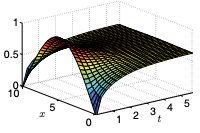
\includegraphics[width=\marginparwidth]{fig76}\captionof{figure}{Solution to 7.3(c)}\label{fig:38}}

\item Modify the Crank-Nicolson program to use boundary conditions
$ \partial T /\partial x = 0$ at the ends. Run with the same initial condition as in
part (a) (which does not satisfy these boundary conditions) and watch
what happens. Zoom in on the plots early in time to see what happens
in the first few grid points during the first few time steps.
\end{enumerate}
\end{problem}